\documentclass[pdflatex,sn-nature,lineno]{sn-jnl}
\usepackage{graphicx}
\usepackage{multirow}
\usepackage{amsmath,amssymb,amsfonts}
\usepackage{booktabs}
\hypersetup{colorlinks=true,allcolors=blue}
\theoremstyle{thmstyleone}
\raggedbottom
\begin{document}
\title[Evaluating LLM-Based Credit Rating Systems]{Evaluating LLM-Based Credit Rating Systems: A Pre-Registered Specification-Curve Analysis}
\author[1]{\fnm{Samir} \sur{Chincholikar}}\email{samir.chincholikar@gmail.com}
\author*[1]{\fnm{Robin} \sur{Chawla}}\email{robin.chawla.cse14@iitbhu.ac.in}
\affil[1]{\orgname{Independent researcher}, \orgaddress{\city{New York}, \country{USA}}}
\abstract{LLMs are increasingly used to support credit assessments, but it is unclear whether
elicitation choices merely reveal a stable credit view or shape the rating. We examine this with a
pre-registered specification-curve design that holds fundamentals fixed while varying how the assessment
is elicited. A fixed 90-item battery spans a balanced grid of provider, model version, temperature,
prompt paraphrase, output format, few-shot exemplars, and presentation, with three seeds
(8{,}640 elicitations, two providers); credit-health profiles use a pre-specified Altman Z$''$
benchmark. Our estimand is stability, not accuracy. No controllable axis accounts for more than about
5\% of rating variance, and pure run-to-run (seed) variation contributes about 8\% (the $\sim$25\%
model residual also absorbs unmodeled interactions). Instability persists even under deterministic
execution (permutation $p=0.001$).
Cross-specification agreement stays limited at every resolution: Fleiss' $\kappa$ reaches at most 0.49
even for the investment-grade/high-yield split, for which 25.2\% of matched pairs disagree; switching or
pooling providers does not remove it. Modal calls imply 53.5\% portfolio turnover, and a post-hoc recast
swings the same \$45 billion book between \$2.0 and \$4.1 billion of Pillar-1 capital. A complementary arm
of 31 anonymized, perturbed real issuers under a decontamination gate shows the same instability.
Elicitation specification is a material source of model risk.}
\keywords{large language models, credit ratings, specification-curve analysis, model risk, reproducibility, investment grade}
\maketitle

\section{Introduction}
Large language models (LLMs) are increasingly used as an analytic tool in finance, including for
financial-statement interpretation, risk assessment, investment recommendations, and credit analysis
\cite{hens2025risk}. In such applications a user usually provides financial information and asks
the model to make a judgment such as a credit rating, risk category, or trading recommendation. Implicit
in such use is the presumption that the model has a sufficiently stable underlying assessment, and that
reasonable changes to the phrasing of the question simply reveal that assessment. If this assumption is
correct, then choices such as prompt wording, output format, sampling temperature, or model provider are
mostly procedural. If it does not hold, then these choices are embedded in the measurement process
itself.

This distinction is of particular importance for credit evaluation. Credit ratings are categorical
decisions with economically important cut points. The investment-grade/high-yield split influences index
eligibility, ratings-based investment mandates, treatment of collateral, covenant provisions, cost of
financing, and regulatory capital. A model that reaches different assessments because the same financial
information is presented under a different but defensible elicitation specification can lead to materially
different downstream decisions even when the underlying firm fundamentals are unchanged. In our
experiments, around 25\% of matched elicitation pairs place the same credit profile on opposite sides of
the investment-grade/high-yield boundary. The key question we ask is therefore not whether an LLM can
produce a plausible credit rating, but whether the rating is sufficiently stable when reasonable
elicitation choices change.

Prompt sensitivity and run-to-run variability in LLMs have been well documented in computer science
\cite{atil2024nondeterminism,kaplan2020scaling}, and recent work has shown related variability in
LLM-generated financial recommendations \cite{chon2025variability}. But three questions remain
unresolved for high-stakes credit applications. First, it is unclear how large this
instability is in the units used by credit practitioners, rather than generic measures of textual
variation. Second, the variation observed may be due to a small number of controllable design choices,
in which case the instability could be mitigated through an appropriate choice of prompt or model
configuration, or it may signal a broader noise floor that persists across the elicitation process. Third,
evaluation using real firms poses a further challenge: general-purpose LLMs may recognize issuers from
publicly available financial information, making it hard to distinguish independent credit assessment
from memorized issuer knowledge.

We address these questions using a pre-registered specification-curve design based on the
multiverse-analysis literature \cite{simonsohn2020specification,steegen2016multiverse}.
Specification-curve analysis considers a single defensible analytical pipeline as a member of a larger
family of reasonable specifications and tests whether the substantive result depends on the particular
choice. Related approaches have been used to study researcher degrees of freedom and annotation
variability \cite{camuffo2026variance}. We extend this logic to machine elicitation, where the
elicitation specification is varied systematically while the financial information and the underlying
task are held fixed. The distribution of ratings obtained is a direct measure of the dependence of the
machine-generated credit opinion on the way it is asked.

In the main experiment, we fix the number of items to 90 and pre-register a grid of elicitation choices
over model provider, model version, temperature, prompt paraphrase, output format, few-shot exemplars,
and answer presentation. The design comprises 8{,}640 planned elicitations across two providers
over three repeated seeds. The financial profiles of the credit-health items are built on a pre-specified
Altman Z$''$ accounting-based benchmark \cite{altman1968}. The benchmark provides a fixed, independently
computable reference for credit health, whereas the elicitation specification varies. Our principal
estimand is therefore not rating accuracy but \emph{stability across specifications}.

The paper makes four contributions. First, we measure the sensitivity of machine-generated credit
ratings to the specification and decompose the rating variation into variation across firm
characteristics, variation due to the elicitation process, variation across providers, and residual
run-to-run variation. This allows us to distinguish instability that could reasonably be addressed by
improved specification choices from variation that remains as a more general noise floor. Second, we
study the persistence of the instability under two natural remedies, deterministic execution and provider
selection, and we measure agreement at different rating resolutions, from the full letter scale to the
investment-grade/high-yield split, to determine whether a stable credit opinion emerges after coarsening
the rating scale. Third, we convert the observed instability into economically interpretable quantities:
rating-boundary migration, portfolio turnover, implied credit-spread variation, and an illustrative
regulatory-capital recast. These analyses relate specification sensitivity to the kinds of decisions that
credit ratings are generally used for. Fourth, we test the persistence of the results outside the
constructed battery while explicitly addressing contamination from model memorization. We compile a set
of 31 U.S. business-to-business issuers with disclosed agency ratings, anonymize the profiles, perturb
all dollar values by an issuer-specific multiplicative factor that preserves financial ratios, and employ
a pre-registered fingerprinting gate to test whether the issuer remains identifiable from the financial
information; identification drops from 22\% with unperturbed profiles to 2.9\% after decontamination.

\section{Related work}
\subsection{Prompt sensitivity and non-determinism in large language models}
Large language models are built on transformer-based foundation models, and their output depends not only
on the information provided to them but also on how that information is elicited
\cite{vaswani2017attention,devlin2019bert,bommasani2021foundation}. Prior work has demonstrated that
semantically irrelevant or substantively minor changes to prompt construction---such as paraphrasing,
answer format, ordering of options, and sampling configuration---can produce materially different outputs
even when the underlying task is unchanged \cite{atil2024nondeterminism,sclar2024formatspread}.
Non-determinism can also be observed in settings intended to produce deterministic responses
\cite{atil2024nondeterminism}.

These results pose a significant measurement challenge for empirical applications of LLMs. If conclusions
are sensitive to a single wording of a prompt, then an observed model response could be an artifact of
the elicitation specification rather than a stable underlying assessment. Mizrahi et
al.\ \cite{mizrahi2024multiprompt} demonstrate how single-prompt evaluation can produce fragile
conclusions and argue for evaluation across multiple prompt formulations. In finance, Chon et
al.\ \cite{chon2025variability} likewise find large variation in stock recommendations produced by LLMs
depending on the prompting and model choice.

\subsection{Multiverse analysis and specification curves}
Empirical results often depend on a set of reasonable analytical choices rather than a single, uniquely
correct specification. The problem has been described as the ``garden of forking paths,'' in which
several defensible decisions can lead to different reported results even in the absence of intentional
specification search \cite{gelman2013garden,simmons2011false}. Multiverse analysis and
specification-curve analysis tackle this problem by assessing the effect across a specified set of
reasonable analytical specifications rather than a single chosen pipeline
\cite{steegen2016multiverse,simonsohn2020specification}.

Specification-curve analysis is particularly useful when the emphasis is on how sensitive a result is to
the choices made by the researcher. The approach examines the distribution of outcomes over the entire
set of defensible specifications, rather than asking whether a given specification leads to a desired
outcome. Similarly, Camuffo et al.\ \cite{camuffo2026variance} introduce a variance-aware approach for
LLM-assisted management annotation, underlining the importance of accounting for the variability
introduced by machine-generated annotations.

We extend this framework to LLM elicitation. We treat each combination of the model and the prompting
choices as one specification, while holding the financial information provided to the model fixed. We
treat the LLM as the estimator under study, and the specification curve that arises
measures the degree to which the inferred credit assessment varies solely due to reasonable choices in
how that assessment is solicited.

\subsection{Large language models for finance, credit, and supervision}
LLMs are increasingly employed for financial tasks that were previously the preserve of specialist
judgment, traditional statistical models, or structured quantitative systems. General-purpose
\cite{brown2020gpt3,ouyang2022instruct,achiam2023gpt4} and finance-specific
\cite{wu2023bloomberggpt,xie2023pixiu} language models have been evaluated for financial-statement
analysis \cite{kim2024fsa}, return prediction \cite{lopezlira2023chatgpt}, analysis of central-bank
communication \cite{hansen2024fedspeak}, risk profiling \cite{hens2025risk}, banking supervision
\cite{garciallorente2026banking}, and credit-rating prediction \cite{drinkall2025forecasting}.

Much of this literature evaluates \emph{capability}: whether an LLM can extract useful financial
information, produce accurate forecasts, classify firms, or approximate expert judgments. For instance,
recent work on credit-rating forecasting compares generative LLMs with established predictive approaches
and finds that conventional methods can retain an accuracy advantage \cite{drinkall2025forecasting}.
These studies concern whether the model performs the task well.

Our question comes before that comparison. An LLM-generated credit assessment should be sufficiently
reproducible under reasonable elicitation choices to be interpretable as a meaningful measurement. A
model can appear accurate under one prompt and output a materially different rating under another equally
defensible prompt. We therefore emphasize \emph{stability versus capability}: whether the credit opinion
itself is unchanged when the information being evaluated is unchanged but the elicitation specification
differs.

\subsection{Credit ratings, economic consequences, and model risk}
Quantitative credit-risk assessment has a long history. Altman's bankruptcy-prediction framework
\cite{altman1968} and later probabilistic approaches such as Ohlson's model \cite{ohlson1980} showed that
accounting information contains systematic signal about corporate financial distress. Credit ratings
encode economically relevant differences across firms, and disagreement among human rating agencies has
been studied as a meaningful feature of the credit-rating process itself
\cite{cantorpacker1997,kligersarig2000,tang2009}.

Rating stability matters because shifts in rating categories can influence financing terms and
institutional choices. Rating differences are associated with borrowing costs and
market pricing \cite{kligersarig2000,tang2009,cornaggia2018}, and migration across the
investment-grade/high-yield boundary can have particularly important implications for investment
mandates, portfolio composition, and capital treatment. On the regulatory side, the Basel standardized
approach maps external credit assessments into risk weights for capital calculations
\cite{bcbs2019cre20}, and supervisory exercises have documented considerable dispersion in risk-weighted
assets even for common portfolios \cite{bcbs2013rcap}.

These concerns connect LLM elicitation to the broader literature on model risk. Under supervisory
guidance, models must be validated, their limitations understood, and the uncertainty in their outputs
appropriately characterized \cite{srletter2011}. If the elicitation specification for an LLM-generated
credit rating changes the rating materially, then the specification itself becomes part of the model-risk
environment. Our work ties these literatures together by directly measuring that instability and
quantifying it not only through statistical disagreement but also through rating migration, portfolio
turnover, spread implications, and regulatory-capital translations.

\section{Results}
The pre-registered design assesses the stability of ratings across two providers (OpenAI and Google),
each evaluated at a current and a prior model snapshot (four snapshots in total), giving balanced coverage
across providers, versions, and the elicitation axes.

\subsection{Sources of rating variation}
We first consider the source of variation in the machine-generated credit rating. An
analysis-of-variance decomposition of the full letter-rating rank (ordinary least squares with Type-II
sums of squares) attributes variance to the firm profile, individual elicitation-design axes, the
provider-by-item interaction, and residual run-to-run variation.

As expected, the firm profile explains most of the observed variance, about 65\% (95\% CI 54--72\%),
indicating that the models respond strongly to differences in the underlying financial information. But
the remaining variation is important because the financial information is constant within each item. No
individual controllable elicitation choice explains more than about 5\% of rating variance; the largest
measured design-axis contribution is answer presentation (4.6\%), the model-provider main effect
contributes only 0.3\%, and the provider-by-item interaction accounts for about 1.4\%. The OLS residual
is $\sim$25\%; separating it, pure within-cell seed variation accounts for only 8.1\% of total variance
(95\% CI 6.4--10.8\%), while the remaining $\sim$17\% reflects unmodeled interactions. Run-to-run
sampling noise is therefore a real but minority component (Table~\ref{tab:var}).

These results indicate that specification sensitivity is not concentrated in a single elicitation choice
that could be avoided by simply selecting a preferred prompt, format, or provider. Instead, the observed
instability is spread across the elicitation process, with variation across repeated calls much larger
than that attributable to any single controllable axis.

The same pattern appears in the specification curve (Fig.~\ref{fig:speccurve}). The three seeds are
pooled, and each point is a pre-registered specification, ordered by benchmark-consistent credit-band
accuracy against the frozen Altman Z$''$ reference. Even when the underlying firm profiles are identical,
performance varies substantially across defensible specifications, with roughly 56\% of the
specifications falling on opposite sides of the pre-registered majority-accuracy threshold. The
specification curve therefore demonstrates that conclusions drawn from a single elicitation configuration
do not necessarily generalize to other plausible configurations.

\begin{figure}[t]\centering
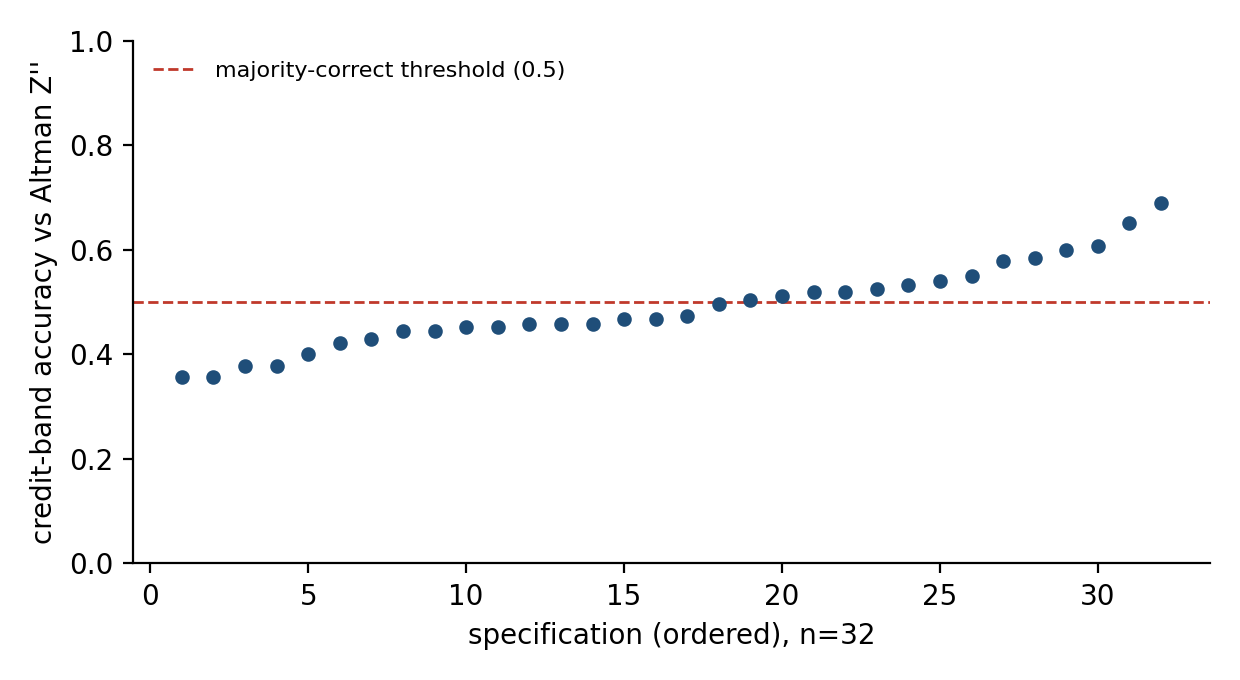
\includegraphics[width=0.82\textwidth]{fig_spec_curve.png}
\caption{Specification curve of the machine credit rating. Each point is one of the pre-registered
specifications (three seeds pooled), ordered by majority-correct credit-band accuracy against the
Altman Z$''$ benchmark. Accuracy ranges widely across specifications despite identical firm
fundamentals, and roughly half reverse the pre-registered accuracy verdict (specification-curve flip
share $\approx0.56$)---the multiverse the method is named for.}
\label{fig:speccurve}
\end{figure}

\begin{table}[t]\centering
\caption{Variance shares of the machine credit letter-rank (OLS decomposition with Type-II ANOVA). Every
controllable design choice is small relative to run-to-run noise.}\label{tab:var}
\begin{tabular}{lr}\toprule
Component & Variance share \\\midrule
Item (firm profile) & 64.9\% (53.9--72.3\%) \\
Residual (total) & 25.2\% \\
\quad --- pure within-cell seed variation & 8.1\% (6.4--10.8\%) \\
\quad --- other unexplained (unmodeled interactions) & $\sim$17\% \\
Answer presentation ($A_7$, largest design axis) & 4.6\% \\
Provider $\times$ item interaction & 1.4\% \\
Model provider ($A_1$, main effect) & 0.3\% \\\bottomrule
\end{tabular}\end{table}

\subsection{Specification fragility under deterministic execution}
One explanation of this residual variation is that some model providers do not fully honor a requested
temperature of zero. If so, the observed instability might largely reflect stochastic sampling rather
than sensitivity to the elicitation specification per se.

We therefore perform the pre-registered determinism test and restrict the analysis to the
provider-setting combination for which the returned metadata confirm deterministic execution: Google at
temperature 0. This subgrid removes repeated-call sampling variation but retains substantial
specification dependence. In it, 62.5\% of specifications fall on opposite sides of the majority-accuracy
threshold, and benchmark-consistent credit-band accuracy ranges from 0.36 to 0.69 across deterministic
prompt configurations.

A one-sided label-permutation test rejects the null of specification invariance. Across 999 permutations,
no permuted labeling produced a between-specification spread as large as the observed statistic, giving
$p=(k{+}1)/(n{+}1)=0.001$. Deterministic execution thus removes run-to-run jitter but does not eliminate
sensitivity to prompt and presentation choices; indeed, the specification-curve flip share within the
deterministic subgrid is higher than the pooled estimate. The instability therefore cannot be ascribed
solely to stochastic sampling.

\subsection{Agreement within and between providers}
The small provider main effect might suggest that provider choice does not matter much. Direct agreement
comparisons reveal a more complex pattern.

Within-provider agreement is consistently higher than cross-provider agreement in the two model families with
full current-and-prior snapshot coverage. Within a single provider, 82.5\% of identical firm profiles
agree at the three-way credit-band level, but only 64.4\% agree across providers. At the full
letter-rating level, agreement across providers falls to 11.1\% from 30.4\% within providers.

These findings are consistent with the variance decomposition. Providers respond differently to specific
firm profiles, creating a provider-by-item interaction. The interaction does not appear to reflect a constant
directional shift in ratings; a simple global adjustment does not allow one provider to be
characterized as systematically more conservative or more generous than another. The disagreement is
issuer-specific.

This distinction is important operationally. Changing vendors does not provide a predictable correction
to the rating of a specific firm, and aggregating outputs across vendors does not remove the underlying
specification dependence. Vendor diversification therefore does not resolve the conceptual measurement
problem or the need to characterize uncertainty across elicitation specifications.

\subsection{Stability across rating resolutions}
Credit ratings are inherently hierarchical. A model may not reproduce an exact letter grade yet still
express a stable broader assessment. We therefore assess cross-specification agreement as we move from
the full 21-grade letter-rating scale to notch categories, three broad credit bands, and the binary
investment-grade/high-yield distinction.

Agreement improves as the scale is coarsened but does not become fully stable. Raw cross-specification
agreement is approximately 16\% at the letter level, 34\% at the notch level, 65\% for the three-way
credit band, and 73\% for the investment-grade/high-yield split. Equivalently, matched elicitation pairs
disagree in about 84\%, 66\%, 35\%, and 27\% of comparisons, respectively (Fig.~\ref{fig:ighy}).

The same conclusion follows from chance-corrected agreement. Fleiss' $\kappa$ is 0.10 at the full letter
scale, 0.21 at the notch level, 0.43 for the three-way band, and reaches a maximum of only 0.49 for the
investment-grade/high-yield split (Fig.~\ref{fig:kappa}). No evaluated rating resolution meets the
conventional threshold for substantial agreement ($\kappa=0.60$).

The instability is not caused by the models collapsing to a narrow set of central ratings. All 21 letter
grades are used across the experiment, and scale-usage entropy is 3.89 of a maximum 4.39 bits. The models
therefore use the available rating scale extensively but do not reproduce the same assessment
consistently across specifications.

The most economically consequential result appears at the coarsest resolution. Even when all finer
distinctions are dropped and only the investment-grade/high-yield classification is retained, 25.2\% of
matched elicitation pairs place the same firm profile on opposite sides of the boundary. Coarsening
reduces specification sensitivity but does not eliminate it.

\begin{figure}[t]\centering
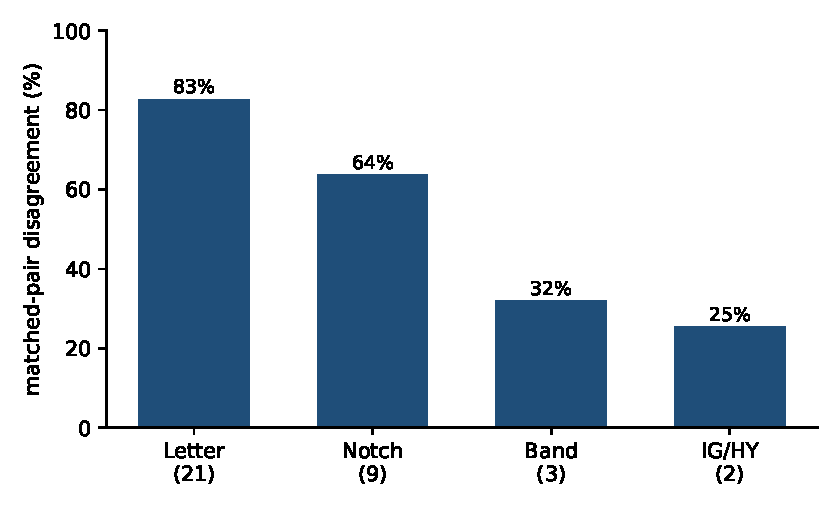
\includegraphics[width=0.66\textwidth]{figure1_ighy.pdf}
\caption{Share of matched elicitation pairs whose credit verdicts differ, by rating granularity, where
the two elicitations of a firm may differ on any grid axis (provider, model version, temperature,
paraphrase, format, few-shot, presentation) and seed. Even at the coarse investment-grade/high-yield
split---the most consequential line in credit---25\% of matched pairs disagree.}\label{fig:ighy}
\end{figure}
\begin{figure}[t]\centering
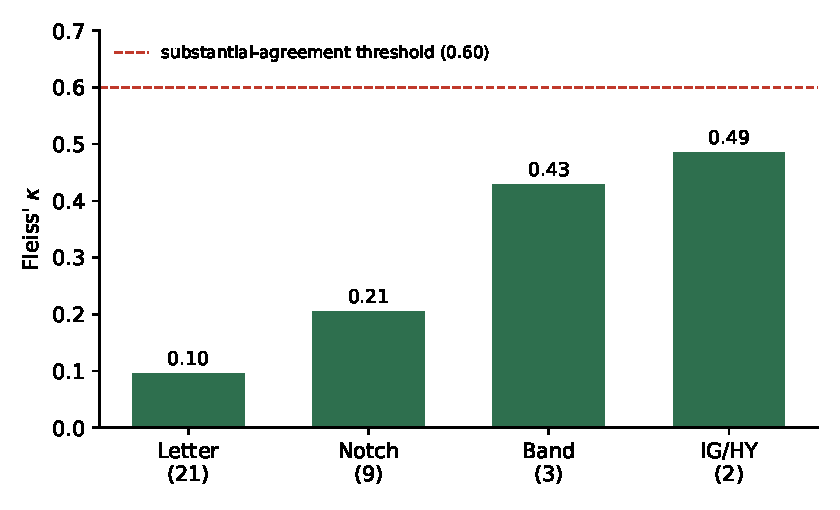
\includegraphics[width=0.62\textwidth]{figureA_kappa.pdf}
\caption{Chance-corrected cross-specification agreement (Fleiss $\kappa$) by granularity; agreement
never reaches the $\kappa=0.6$ substantial-agreement threshold, peaking at 0.49 on the IG/HY split.}
\label{fig:kappa}
\end{figure}

\subsection{Economic implications of elicitation instability}
Statistical disagreement is economically important when alternative specifications produce decisions on
opposite sides of consequential credit boundaries. We translate the observed rating instability into
three decision-relevant quantities: investment-grade/high-yield migration, portfolio turnover, and
illustrative spread and capital implications.

For each credit-health profile we draw two elicitations from its observed specification distribution,
allowing the pair to differ on any elicitation axis and on seed. We then compute, for each firm, the
probability that the two resulting ratings fall on opposite sides of the investment-grade/high-yield
boundary, and average across profiles. This per-comparison flip probability is one minus the
Gini--Simpson concentration of the firm's binary IG/HY outcomes.

This yields an investment-grade/high-yield flip rate of 25.2\% (95\% CI 19.7--31.2\%): more than a
quarter of matched ratings for the same underlying credit profile disagree on which side of the
investment-grade boundary the profile falls.

The implication for the directional task is similar. A strategy that mechanically follows the modal
buy/hold/sell call across specifications would incur 53.5\% implied turnover (95\% CI 47.4--58.9\%) due
solely to elicitation choices. With the financial inputs unchanged, this turnover reflects specification
instability rather than new economic information.

We also offer two post-hoc economic calibrations. Across all profiles, the median within-name
spread range is about 275 basis points under the rating-spread schedule of Cornaggia et
al.\ \cite{cornaggia2018}, inflated by names saturating in the CCC region; for non-saturating profiles
the median range is about 261 basis points, with a floor near 42 basis points. Mapping
each specification's rating through the Basel standardized external-ratings risk-weight framework
\cite{bcbs2019cre20} for a single hypothetical \$45 billion equal-weight corporate portfolio, the
resulting Pillar-1 minimum-capital requirement---driven only by the elicitation specification---ranges
from approximately \$2.0 billion to \$4.1 billion (median \$3.1 billion). Two randomly drawn specifications differ by about
\$0.65 billion on average, or 20.5\% of the median computed capital requirement---comparable to the
$\sim$20\% relative dispersion the Basel RCAP exercise found across internal-model banks holding
identical portfolios \cite{bcbs2013rcap}. Although these spread and capital calculations are explicitly
post-hoc calibrations rather than confirmatory tests, they indicate that the magnitude of
specification-induced rating dispersion is economically non-trivial (Table~\ref{tab:frag}).

\begin{table}[t]\centering
\caption{Fragility in decision and economic units. Parenthetical values are 95\% confidence intervals
(issuer-clustered percentile bootstrap).}\label{tab:frag}
\begin{tabular}{lr}\toprule
Quantity & Result \\\midrule
Specifications flipping majority credit \emph{band} verdict (pooled / determ.) & $\sim$56\% / 62.5\% \\
Credit-band accuracy range, honored-determinism subgrid & 0.36--0.69 \\
Permutation test, determinism subgrid & $p=0.001$ \\
Within- vs cross-vendor agreement (band / letter) & 82.5/64.4 $\cdot$ 30.4/11.1 \\
Max chance-corrected agreement (Fleiss $\kappa$, IG/HY) & 0.49 (no scale $\geq0.6$) \\
Per-comparison IG/HY boundary flip & 25.2\% (95\% CI 19.7--31.2\%) \\
Implied turnover (modal-call instability) & 53.5\% (95\% CI 47.4--58.9\%) \\
Implied spread range per name (non-saturating / median) & $\sim$261 / $\sim$860 bps \\
Pillar-1 capital range, same \$45bn book (post-hoc cut) & \$2.0bn -- \$4.1bn \\\bottomrule
\end{tabular}\end{table}

\subsection{Robustness on decontaminated real issuers}
The constructed battery provides the controlled context in which to identify elicitation instability, but
a key external-validity concern is whether similar behavior appears for real firms. Direct evaluation on
real issuers raises a further methodological problem: an LLM may recognize a company from publicly
available financial figures even when the company name is removed.

We test this possibility first, before using real issuers as a robustness sample. When presented with anonymized
but otherwise unchanged financial profiles, Gemini-Flash correctly identifies about 22\% of the selected
mid-cap issuers from their financial numbers alone. This shows that anonymizing the issuer name does not
guarantee that an LLM makes an independent credit assessment rather than relying on memorized issuer
information.

The pre-registered fingerprinting gate lowered the issuer-identification rate from 22\% to 2.9\%, below
the pre-specified 5\% threshold. The decontaminated firms are then rated on a frozen 12-specification grid
at three seeds, and the constructed battery is re-rated under exactly the same specification grid to
provide a matched comparison.

The real-firm WATCH-stratum flip share is 0.226 (95\% CI 0.147--0.308), relative to 0.318 (95\% CI
0.223--0.406) for the matched constructed battery. The estimated difference is $-0.091$ (95\% CI $-0.213$
to $0.032$; Table~\ref{tab:realarm}). The difference is not statistically distinguishable from zero;
however, the pre-registered two-one-sided-tests (TOST) equivalence test at the $\pm0.15$ margin does not
establish quantitative equivalence ($p=0.179$), consistent with limited power at 16 real and 15 battery
WATCH observations.

The appropriate conclusion is therefore narrower than numerical equivalence: substantial specification
instability remains observable in decontaminated real issuers under the same elicitation conditions. The
real-firm point estimate is somewhat lower than the matched battery's, but the available sample is too
small to determine whether that difference is a stable population difference. As a separate descriptive
reference, machine-generated credit bands match the disclosed agency ratings about 54\% of the time.

\begin{table}[t]\centering
\caption{Real-firm arm: 31 decontaminated business-to-business issuers, agency-rating benchmark.
Parenthetical values are 95\% confidence intervals (issuer-clustered percentile bootstrap).}
\label{tab:realarm}
\begin{tabular}{lr}\toprule
Quantity & Result \\\midrule
Fingerprint identification, naive (exact figures) & 22\% \\
Fingerprint identification, decontaminated (gate) & 2.9\% \\
WATCH-stratum flip-share, real arm & 0.226 (0.147--0.308) \\
WATCH-stratum flip-share, battery (same 12 specs) & 0.318 (0.223--0.406) \\
Difference (real $-$ battery), 95\% CI & $-0.091$ ($-0.213$, $0.032$) \\
Equivalence test (TOST, $\pm0.15$ margin) & $p=0.179$ (not established; underpowered) \\
Interpretation & substantial instability persists; equivalence not established \\
Machine band vs.\ disclosed agency rating (descriptive) & 54\% \\\bottomrule
\end{tabular}\end{table}

\section{Discussion}
We examine whether an LLM-generated credit rating can be treated as a stable assessment of a firm's
financial health or whether it depends heavily on how that measure is elicited. The main finding of the
pre-registered specification curve is that substantial instability remains even after controlling for the
underlying financial information. As expected, firm characteristics explain most of the total variation
in ratings, but the residual variation due to elicitation and repeated calls is large enough to change
economically meaningful decisions.

The variance decomposition clarifies the origin of this instability. No single controllable design choice
explains more than $\sim$5\% of rating variance; of the $\sim$25\% OLS residual, only about 8\% is pure
run-to-run seed variation, the remainder being structured but unmodeled sensitivity to the elicitation
specification. This distinction matters because it implies that the instability is neither reducible to a
single tunable knob nor dismissible as sampling noise, and cannot be
resolved by selecting a preferred prompt formulation, output format, temperature, or provider. No single
elicitation parameter dominates the observed instability; instead, the same financial
information can produce meaningfully different credit assessments under multiple reasonable
specifications.

The real-issuer experiment complements, rather than substitutes for, this identification strategy.
Crucially, it first demonstrates that direct evaluation on anonymized real firms is not automatically
clean: a model identifies around 22\% of the unperturbed issuers from financial information alone. After
issuer-specific scaling and screening, the fingerprint rate falls to 2.9\%, and substantial
specification instability is still observed in the real-firm arm under this decontamination gate. The
real and constructed WATCH estimates are not shown to be quantitatively equivalent, and the sample is too
small to support such a claim; nevertheless, the qualitative pattern persists and suggests that the main
finding is not confined to the controlled battery.

The fingerprinting result also has implications beyond the credit-rating experiment at hand. Public
companies' financial information is widely disseminated and may have been included in the training data
of general-purpose LLMs. Removing company names does not necessarily remove issuer identity from an
evaluation: if a model can infer the issuer from the precise financial numbers, then a judgment that
appears to be based on the inputs may also draw on memorized information about that company. Perturbation
combined with explicit identification testing is a practical way to mitigate this risk when evaluating
LLMs on public financial entities.

Taken together, the results suggest that a credit rating produced by an LLM should not be interpreted as a
specification-invariant point estimate. Each response is one realization from a broader distribution induced
by the elicitation procedure. This does not imply that LLMs cannot contribute to credit analysis, and the
present study does not assess whether their ratings are more or less accurate than established
credit-assessment methods. Rather, a prerequisite for reliable use is to characterize the uncertainty
associated with reasonable elicitation choices before treating a point rating as a stable model output.

This interpretation ties directly to model-risk management. Model outputs used in consequential financial
decisions are generally expected to be validated and their uncertainty and limitations understood
\cite{srletter2011}. Our results suggest that, for LLM-based credit assessment, the elicitation
specification itself should be part of that uncertainty assessment. Reporting a single rating without
evaluating its sensitivity to plausible specifications can convey a false sense of precision. Repeated
elicitation, related stability diagnostics, or specification curves therefore provide a more informative
representation of machine-generated credit opinions than a single prompted response.

\noindent\textbf{Limitations.} These findings have several limitations that bound their scope. First, the study considers two providers
and the specific model snapshots and configurations included in the pre-registered design; the
results should therefore be viewed as evidence of how the evaluated systems behave, not as a universal
numerical estimate for all current or future LLMs.

Second, the main identification sample is a fixed 90-item constructed battery, with 45 profiles in the
credit-health task and 45 in the directional task. Repeated specifications increase coverage of the
elicitation space but not the number of independent underlying firm profiles, so the flip rates and
variance estimates remain sample statistics for the battery considered.

Third, the real-firm arm comprises 31 U.S. mid-cap business-to-business issuers selected under the
decontamination design. This sample checks external validity but is much smaller than the controlled
battery at the relevant strata; in particular, the WATCH-stratum comparison lacks the power to detect the
pre-specified equivalence margin, and quantitative equivalence between the constructed and real-firm
estimates is not established.

Fourth, the study measures stability, not absolute credit-rating capability. The Altman Z$''$ mapping
provides a pre-specified accounting-based benchmark for constructing and evaluating the controlled
credit-health battery, while disclosed agency ratings provide an alternative descriptive reference;
neither is treated as a unique ground-truth credit opinion. Whether generative models can produce more
accurate credit assessments than established statistical, market-based, or agency methods is a separate
research question.

Finally, the spread and regulatory-capital translations are post-hoc calibrations that express observed
rating dispersion in economically interpretable units. They are not pre-registered tests and are not
intended as simulations of a real regulatory or institutional implementation. Within these bounds, the
main stability finding is robust across the specification curve, the deterministic subgrid, the provider
comparison, the rating-resolution analysis, and the decontaminated real-firm arm.

\noindent\textbf{Future directions.} The present design suggests several extensions. Larger and sector-stratified real-issuer samples would
yield more precise estimates of how specification instability varies with firm characteristics and
distance from rating boundaries. Similar designs could test retrieval-augmented or tool-using credit
agents, where access to external information may reduce some forms of uncertainty while adding further
specification choices. Human-in-the-loop workflows could also be explored to determine whether providing
analysts with distributions of machine ratings or specification curves leads to more reliable decisions
than a single model-generated assessment. More broadly, the decontamination procedure could be applied to
other evaluations of financial LLMs involving publicly documented entities: explicitly testing whether an
ostensibly anonymized case remains identifiable, in tasks such as risk assessment, valuation, investment
recommendation, and supervisory analysis, may help separate independent reasoning from memorized entity
knowledge.

Overall, reproducibility in AI-assisted credit assessment cannot be taken for granted from a
single elicitation. Across a pre-registered specification curve, firm fundamentals explain most of the
total variation in machine-generated ratings, but substantial specification- and run-level instability
remains after controlling for the underlying financial information. No single controllable elicitation
choice explains much of this variation, and the instability persists even when the analysis is limited to
verified deterministic execution.

These results are not evidence that LLMs are accurate credit raters, and they do not imply that all
current or future models will exhibit the same level of instability. For the systems studied here they
make a more basic point: the elicitation procedure is part of the measurement. Unless stability with
respect to reasonable elicitation choices has been demonstrated, a machine-generated credit rating should
not be treated as a specification-independent point estimate. In AI-assisted credit analysis, the outcome
includes the specification.

\section{Methods}
\subsection{Design, battery, and benchmark}
The study is designed to measure \emph{elicitation stability}: whether an LLM produces a credit
assessment that is consistent when the underlying financial information is held constant but reasonable
choices in how the assessment is elicited vary. The aim is therefore not to estimate rating accuracy on a
naturally occurring population of firms, but to isolate variation attributable to the elicitation
process.

We use a constructed battery as the main identification environment because it allows firm fundamentals
to be held fixed while the elicitation specification varies, permits balanced representation across
credit-health conditions, and provides a benchmark that can be computed before any model is queried.
Restricting the analysis to public companies would introduce a further source of uncertainty,
because an LLM might identify an issuer from financial information it was exposed to during training. We
therefore use the controlled battery for the main analysis and a separately decontaminated real-firm
sample for a complementary external-validity test.

The battery consists of 90 fixed firm-quarter profiles. Each profile is summarized in a compact financial
statement, including revenue, EBIT, total assets and liabilities, equity, working-capital figures, and
retained earnings. The profiles comprise two equally sized task families: 45 credit-health items, for
which the model produces a credit rating, and 45 directional items, for which the model produces a
buy/hold/sell call. All credit-rating agreement and investment-grade/high-yield analyses use the 45
credit-health profiles; the directional profiles are used only for the portfolio-turnover translation.

For the credit-health task, each profile is associated with a pre-specified Altman Z$''$ accounting-based
reference \cite{altman1968}, computed with coefficients 6.56, 3.26, 6.72, and 1.05 and cutoffs 2.60 and
1.10. The resulting safe, watch, and distress strata each contain 15 observations, evenly distributed
across the 45 credit-health profiles. The Altman mapping provides a deterministic accounting reference
for constructing and stratifying the controlled battery and is not treated as a unique ground-truth
agency rating, because our interest is stability across elicitation specifications rather than absolute
rating accuracy. The benchmark and battery were frozen under a pre-registration hash before any model
query, and an independent post-hoc re-execution from the frozen financial facts reproduces all 45
benchmark classifications.

\subsection{Specification grid and data collection}
We manipulate seven researcher-controlled elicitation dimensions: model provider (OpenAI, Google),
model version (a current and a prior snapshot per provider), temperature (0 or 1.0), prompt paraphrase
(three semantically equivalent formulations), output format (JSON or free-text), few-shot exemplars (zero
or two), and answer presentation (original prose versus a table with reversed option ordering). A
balance-constrained D-optimal fractional design of 32 specifications was generated from an effect-coded
main-effects model with the design seed frozen in advance. Each specification was evaluated over three
seeds. Provider metadata were preserved as returned, including effective generation settings where
available; the requested temperature of 0 was not uniformly honored by providers.

The confirmatory experiment therefore comprises $90\times32\times3=8{,}640$ elicitation cells, of which
8{,}633 returned substantive content. Each call is stored as an immutable JSON record containing the experimental specification, the
returned content, and the available provider metadata. Data collection and analysis are separated: all
confirmatory analyses run only on the frozen response corpus and do not re-query any model.

\subsection{Outcome construction and statistical analysis}
Stored model responses are parsed under three rules---strict, lenient, and tolerant---applied after
collection. Credit ratings are first expressed on the full 21-grade letter scale and then deterministically
aggregated into notch categories, three broad credit bands, and the binary investment-grade/high-yield
classification. This permits examination of stability at increasingly coarse rating resolutions without
additional model calls.

Agreement across specifications is measured with Fleiss' $\kappa$. Within- and cross-provider agreement
is computed on matched firm profiles and seeds, and the contrast between homogeneous and heterogeneous
ensembles is summarized by $\Delta\kappa$ with profile-clustered bootstrap confidence intervals.
Variation in the full letter-rating rank is decomposed by ordinary least squares with Type-II analysis
of variance, with terms for the underlying item, the elicitation-design dimensions, the
provider-by-item interaction, and residual run-level variation.

All analyses are pre-registered unless labelled post-hoc, and inference uses distribution-free resampling
throughout, so no normality assumption is made. Uncertainty for the main quantities is estimated by
percentile bootstrap resampling over the underlying firm profiles rather than over individual model calls,
thereby preserving dependence among repeated elicitations of the same profile. The
investment-grade/high-yield flip rate and the portfolio-turnover estimate use 2{,}000 bootstrap
replicates, and specification-curve quantities use 1{,}000 replicates where applicable; point estimates
are reported with two-sided 95\% confidence intervals. Specification invariance under deterministic
execution is tested on the provider-setting combination whose metadata confirm that temperature was
honored (Google at temperature 0): the observed between-specification spread in credit-band accuracy is
compared with the distribution generated by 999 permutations in a one-sided label-permutation test,
$p=(k{+}1)/(n{+}1)$, where $k$ is the number of permuted statistics at least as extreme as the observed
statistic and $n=999$. The test is one-sided because only an observed spread larger than the permutation
distribution constitutes evidence against specification invariance. For the real-firm robustness
analysis, quantitative equivalence of the real-firm and constructed-battery WATCH-stratum flip shares is
assessed with two one-sided tests (TOST) against a pre-registered margin of $\pm0.15$, based on 16
real-firm and 15 constructed WATCH observations. The significance threshold is $\alpha=0.05$ for all
formal tests. To mitigate the risk of selective reporting within the specification multiverse, we
pre-registered the estimands and specification grid and report the entire specification curve rather than
a selected subset. We reserve ``significant'' for results accompanied by a $p$-value and otherwise use
``substantial'' or ``considerable.''

For the binary IG/HY outcome, the per-comparison flip probability is computed separately for each
credit-health profile from its observed distribution of ratings across the entire elicitation grid, so
that two elicitations may differ on any specification dimension or seed. The resulting pair falls on
opposite sides of the IG/HY boundary with probability equal to one minus the Gini--Simpson concentration
of the profile's binary labels, and the reported flip rate is the average of this quantity over the 45
credit-health profiles.

\subsection{Economic translation}
The economic translations are post-hoc calibrations that express the magnitude of rating instability in
decision-relevant units; they are not confirmatory tests. Portfolio turnover is computed from the 45
directional profiles as the share of positions whose modal buy/hold/sell decision changes across
elicitation specifications. Rating dispersion is transformed into indicative credit-spread variation
using the rating-spread schedule of Cornaggia et al.\ \cite{cornaggia2018} and a cached daily
option-adjusted-spread series. For the regulatory-capital illustration, each specification's rating is
mapped through the Basel CRE20 standardized external-ratings risk-weight schedule \cite{bcbs2019cre20} and
applied to the same hypothetical \$45 billion equal-weight corporate portfolio, so that the capital range
reflects only differences in the elicited rating. The comparison with the Basel Regulatory Consistency
Assessment Programme \cite{bcbs2013rcap} is used only as a magnitude calibration, not as an identity
between the two settings.

\subsection{Real-firm arm}
To test the persistence of specification instability outside the constructed battery, we assemble a
complementary sample of 31 U.S. business-to-business issuers with market capitalizations between \$2
billion and \$15 billion whose most recent Form 10-K discloses a current long-term agency credit rating.
S\&P is the primary rating source; where S\&P ratings are unavailable, Moody's or Fitch ratings are
mapped to a common scale. Each rating is preserved with a verbatim filing quotation, a permanent SEC
document URL, and a document hash.

Because these figures are publicly reported by real issuers, there is a risk of contamination if a model
can identify a company. We therefore first perform a pre-registered fingerprinting test in which the
models are asked to identify issuers from anonymized financial profiles; Gemini-Flash identifies about
22\% of the selected issuers from the original figures, confirming that removing the company name does not
guarantee independence from memorized issuer information. To reduce this risk, every dollar-denominated
quantity for an issuer is multiplied by a single issuer-specific factor sampled from a log-uniform
distribution over $[0.6,1.7]$. The same factor applies to all monetary amounts, so the credit-health
analysis retains the financial-ratio structure while disrupting exact-figure lookup. We also
exclude consumer-facing companies to reduce recognition from highly distinctive public profiles. The
fingerprint-identification rate falls to 2.9\% after perturbation, below the pre-registered 5\%
decontamination threshold.

Each decontaminated issuer is then scored on a fixed 12-specification grid spanning presentation,
provider, prompt paraphrase, and output format, at three seeds, and the constructed battery is re-scored
under the same grid for a matched comparison on the WATCH stratum. This arm uses disclosed agency ratings
as a descriptive real-world reference; the primary comparison is stability across specifications.

\subsection{Reproducibility}
The entire experimental pipeline is archived so that the reported results can be reproduced without
further model calls. The frozen materials comprise the 90-item battery, the specification grid, the
prompt templates, the rating scale, the full 8{,}640-record response corpus, the analysis panel, the
real-firm arm, the analysis code, the generated outputs, and SHA-256 integrity manifests. The complete
set of confirmatory tables, figures, and reported statistics regenerates from a single offline entry
point. Provider API credentials are required only to collect new model responses and are not needed to
reproduce any result reported in this study.

\textbf{Use of generative AI.} Generative AI was used to assist with grammar correction and minor
language edits of the authors' own text, and with software scaffolding, development, and coding of the
analysis and reproducibility pipeline (Anthropic Claude), in all cases under the authors' direction.
Separately, large language models are the object of study in this work---the credit-rating elicitations
under analysis---as described above; every such elicitation is recorded in the specification grid and
frozen corpus. The authors reviewed and verified all such output and take full responsibility for the
content.

\backmatter
\bmhead{Data Availability}
All data and code required to reproduce the study are openly available in a deterministic, offline
reproducibility capsule archived on Zenodo (\url{https://doi.org/10.5281/zenodo.21953935}; MIT license),
mirrored in the source repository at \url{https://github.com/samirrc2/Sensitivity-of-AI-Generated-Credit-Ratings-to-Elicitation-Choices}. Within the capsule, the
\texttt{data/frozen/main/} directory contains the pre-registered 90-item firm battery
(\texttt{battery\_90.json}; 45 credit-health $+$ 45 directional items), the specification grid
(\texttt{grid\_definition.json}), the prompt paraphrases (\texttt{paraphrase\_templates.json}), the
rating scale (\texttt{rating\_scale.json}), and the Basel capital map (\texttt{capital\_map.json});
\texttt{data/raw/main/} holds the complete frozen corpus of 8{,}640 model responses;
\texttt{data/panel/panel.parquet} is the analysis panel built once from that corpus; and
\texttt{data/frozen/realarm/} with \texttt{data/raw/realarm/} contain the decontaminated real-firm arm
(the anonymized perturbed battery \texttt{battery\_real45.json}, the sealed issuer crosswalk, the rating
provenance \texttt{ratings\_provenance.csv} with a verbatim 10-K quotation, permanent SEC URL, and
document hash per issuer, and the arm/comparator/fingerprint model-output panels). The analysis code is
in \texttt{analysis/}, pre-computed outputs and figures in \texttt{results/}, and SHA-256 integrity
manifests in \texttt{manifest/}. A single offline entry point, \texttt{reproduce.sh}, regenerates every
reported number, table, and figure byte-for-byte, with no model calls and no API keys. Issuer identities
in the real-firm arm are anonymized and the sealed crosswalk is withheld; the underlying SEC filings
(Form 10-K and company-facts XBRL) are publicly available through the SEC EDGAR system, with permanent
document URLs listed in \texttt{data/frozen/realarm/ratings\_provenance.csv}.

\bmhead{Code availability}
All collection, panel-construction, and analysis code is released under the MIT license in the same
repository; a single \texttt{reproduce.sh} regenerates every reported number, table, and figure from the
frozen data offline. Provider API keys are required only to re-collect the corpus (not to reproduce any
result) and are not distributed.

\bibliography{references}

\bmhead{Author contributions}
\textbf{S.C.:} Conceptualization, Methodology, Software, Formal analysis, Data curation, Writing --
original draft, Writing -- review \& editing. \textbf{R.C.:} Conceptualization, Validation, Writing --
review \& editing. All authors reviewed and approved the manuscript.

\bmhead{Ethics declarations}
This study did not involve human participants, human tissue, or animal subjects, and used no personally
identifiable or sensitive personal data; ethical approval was therefore not required. The analysis uses
only synthetic firm profiles, publicly available corporate financial disclosures (SEC filings), and the
authors' own model elicitations.

\bmhead{Additional Information}
\noindent\textbf{Competing interests:} S.C. and R.C. each declare no competing interests.\\
\textbf{Funding:} This research received no external funding.
\end{document}
